\documentclass[12pt]{article}
\usepackage[margin=0.5in,paper=a4paper]{geometry} %Shrinking margins to 0.5in
\usepackage[x11names]{xcolor}                     %Additional colors
\usepackage{tikz}
\usepackage[amsbb]{mtpro2}                                %Nicer numbers

%Note about the colors: 
%  The color of the "ray" lines should not be
%  black or gray as on some printers, significant
%  aliasing distorsion becomes visible.

\begin{document}
\thispagestyle{empty} %Please, no page numbers or similar

\begin{center}
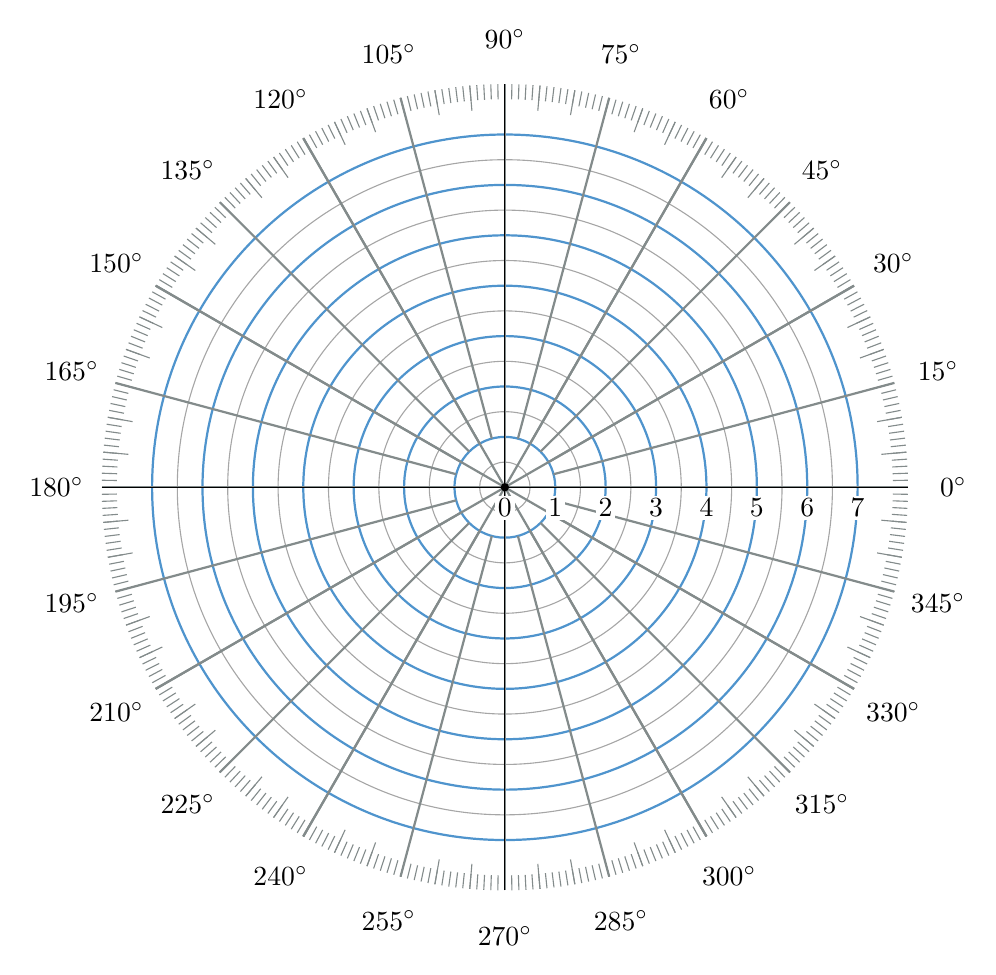
\begin{tikzpicture}[scale=0.64]
%Circles 
\foreach \r in {1, 2,...,7}
\draw[SteelBlue3, thick] (0,0) circle (\r);    
\foreach \r in {0.5, 1.5,...,7}
\draw[gray!70, thin] (0,0) circle (\r);
%1° Rays
\foreach \a in {0, 1,...,359}
\draw[Azure4] (\a:7.7) -- (\a:8);
%5° Rays
\foreach \a in {0, 5,...,359}
\draw[Azure4] (\a:7.5) -- (\a:8);      
%15° Rays
\foreach \a in {0, 15,...,359}
\draw[thick,Azure4] (\a:1) -- (\a:8); 
%30° Rays
\foreach \a in {0, 30,...,359}
\draw[thick,Azure4] (0, 0) -- (\a:8);
%Main rays
\draw (-8,0) -- (8,0);
\draw (0,-8) -- (0,8);
%Angle labels  
\foreach \a in {0, 15,...,359}
\draw (\a: 8.9) node[fill=white,inner sep=.2mm] {$\a^\circ$};
%Central point
\draw[fill=black] (0,0) circle(0.7mm);
%Radius labels (background filled white)
\foreach \r in {0,1,...,7}
\draw (\r,0) node[inner sep=1pt,below=3pt,rectangle,fill=white] {$\r$};
\end{tikzpicture}
\end{center}

\end{document}